\chapter{Data and MC samples}
\label{ch:ana-intro}

\section{Data samples}
The pp collisions at a centre-of-mass
energy of 13~TeV recorded between 2015 and 2017 are used in this search, while the Good-Run-Lists are showed below:
\begin{itemize}
        \scriptsize
\item \texttt{data15\_13TeV.periodAllYear\_DetStatus-v89-pro21-02\_Unknown\_PHYS\_StandardGRL\_All\_Good\_25ns.xml}
\item \texttt{data16\_13TeV.periodAllYear\_DetStatus-v89-pro21-01\_DQDefects-00-02-04\_PHYS\_StandardGRL\_All\_Good\_25ns.xml}
\item \texttt{data17\_13TeV.periodAllYear\_DetStatus-v99-pro22-01\_Unknown\_PHYS\_StandardGRL\_All\_Good\_25ns\_Triggerno17e33prim.xml}
\item \texttt{data18\_13TeV.periodAllYear\_DetStatus-v102-pro22-04\_Unknown\_PHYS\_StandardGRL\_All\_Good\_25ns\_Triggerno17e33prim.xml}
\end{itemize}
The resulting dataset corresponds to an integrated luminosity of 3.2~\ifb, 33.0~\ifb, 44.3~\ifb\ and 58.5~\ifb\ for each Good-Run-Lists, respectively. The total integrated luminosity is 139.0~\ifb. The proton bunch gap equals to 25~ns.


\section{Trigger}
\label{sec:trigger}

\par \MET~triggers is used in 0 and 1 lepton regions and unprescaled single-muon triggers in the 2 lepton region. 
Their thresholds are determined by requiring lowest unprescaled single-muon triggers~\cite{lowest_unprescaled_triggers}. 

\par An offline cut \MET~$>$ 150~GeV is applied as the triggers are not fully efficient in low \MET~region. Since the trigger turn-on curve is not well modeled in MC,
 trigger efficiencies are measured in both data and MC from a single-muon measurement region, and scale factors are calculated to correct
turn-ons in MC to match data in the signal region and the single-muon control region.

\par \METnomu~compensates the online \MET~which is reconstructed using only calorimeter informationin without the contribution of the muon.
Events collected with the muon trigger can be used to measure the trigger turn-on curve of the \MET~trigger. 

\par The efficiencies of \MET~triggers are derived in a single-muon measurement region.
The event selection is same as the selection in the resolved regime in Chapter~\ref{ch:ana-sig}, except for the cut on \met.
The efficiencies are calculated inclusively in the number $b$-jets to allows for a larger statistics in the measurement region.


\par The \MET~trigger efficiency is defined by:

\begin{equation}
\label{eq:trigeff}
\text{efficiency} = \frac{\text{\#Events passed selection AND \MET~trigger requirement}}{\text{\#Events passed selection}}
\end{equation}

\par The efficiencies are calculated for each \MET~trigger separately within the data-taking periods in which it was used, and separately for data and MC.
 The trigger efficiency curves for each \MET~trigger are shown in Fig.~\ref{fig:TrigEff} as a function of \METnomu~to mimic the \MET~topology on trigger level.

\begin{figure}[tb!]
	\centering
	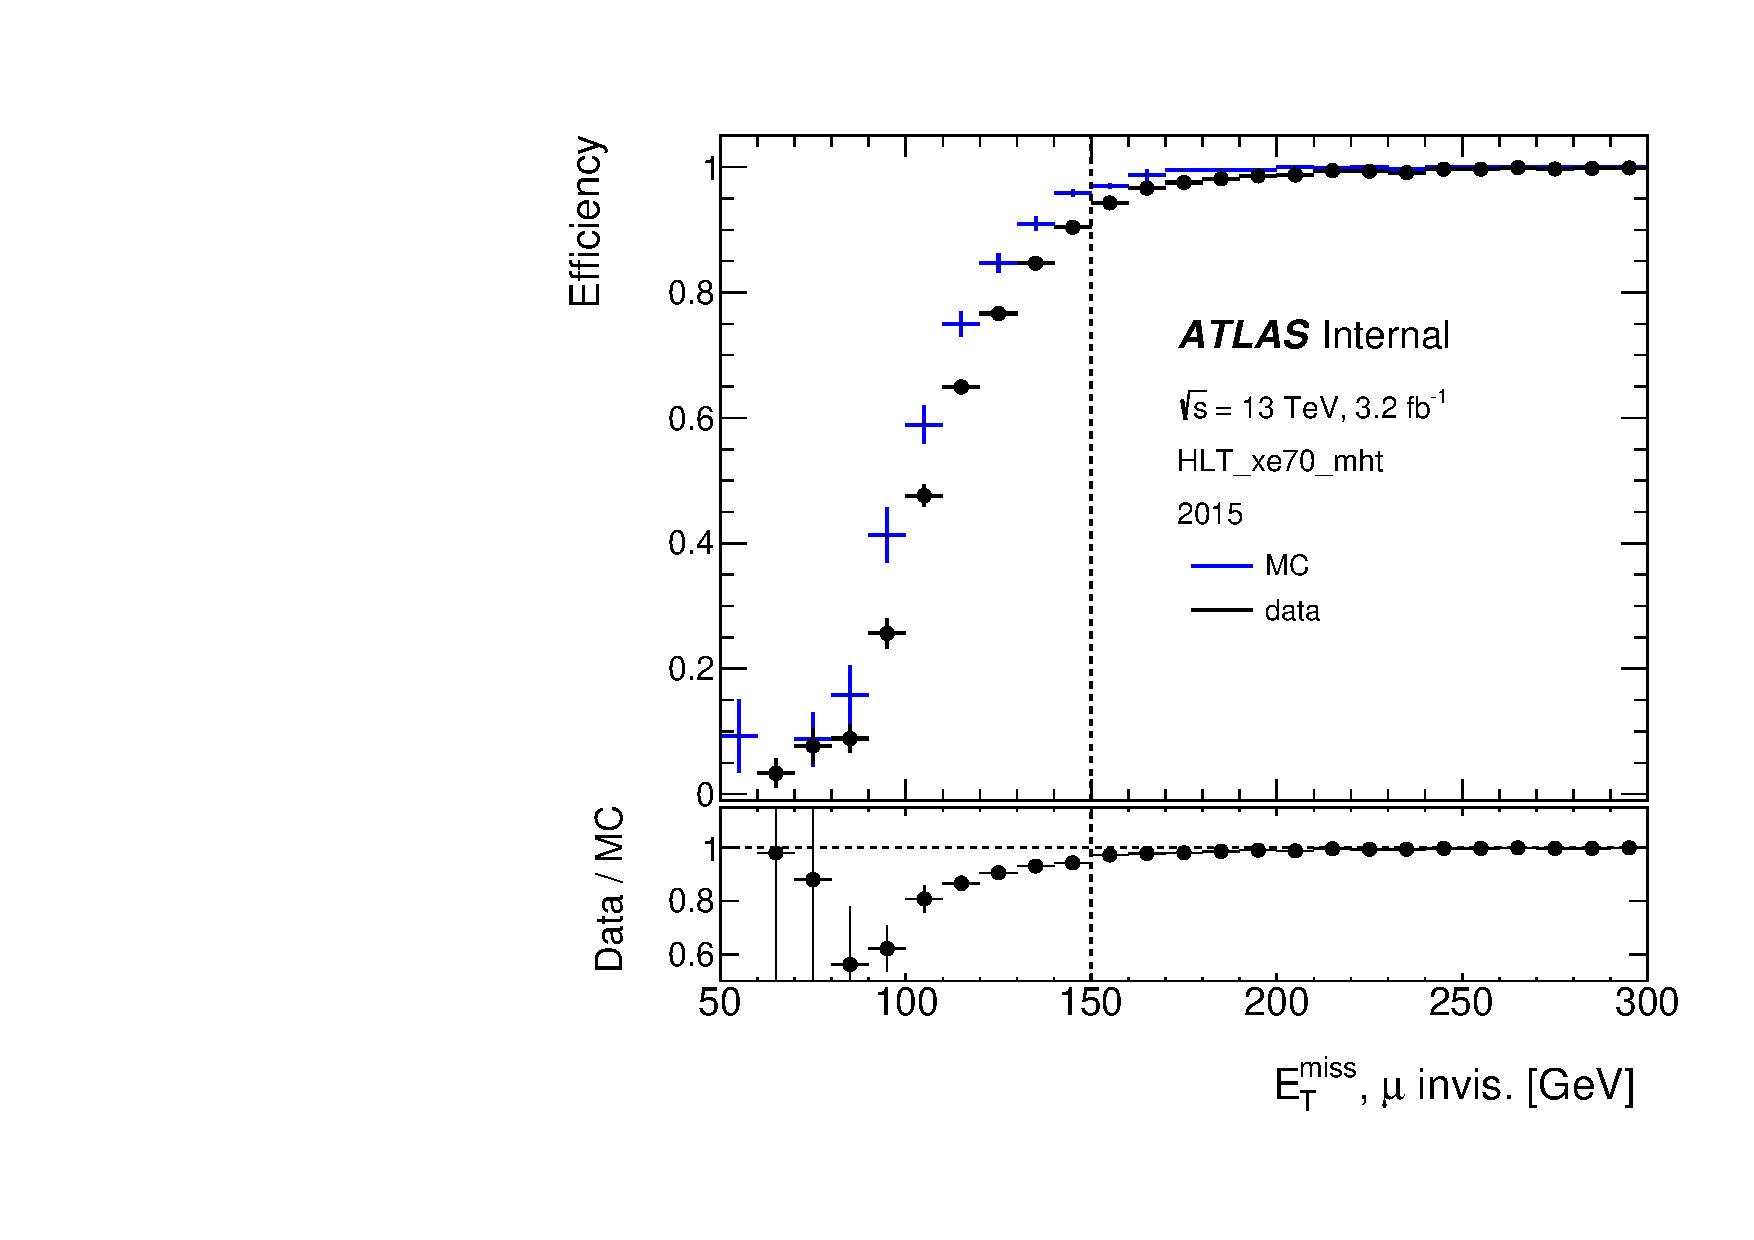
\includegraphics[width=0.45\textwidth]{chapters/c6/fig/METTriggerCalibration/efficiecy_HLT_xe70_mht.pdf}
	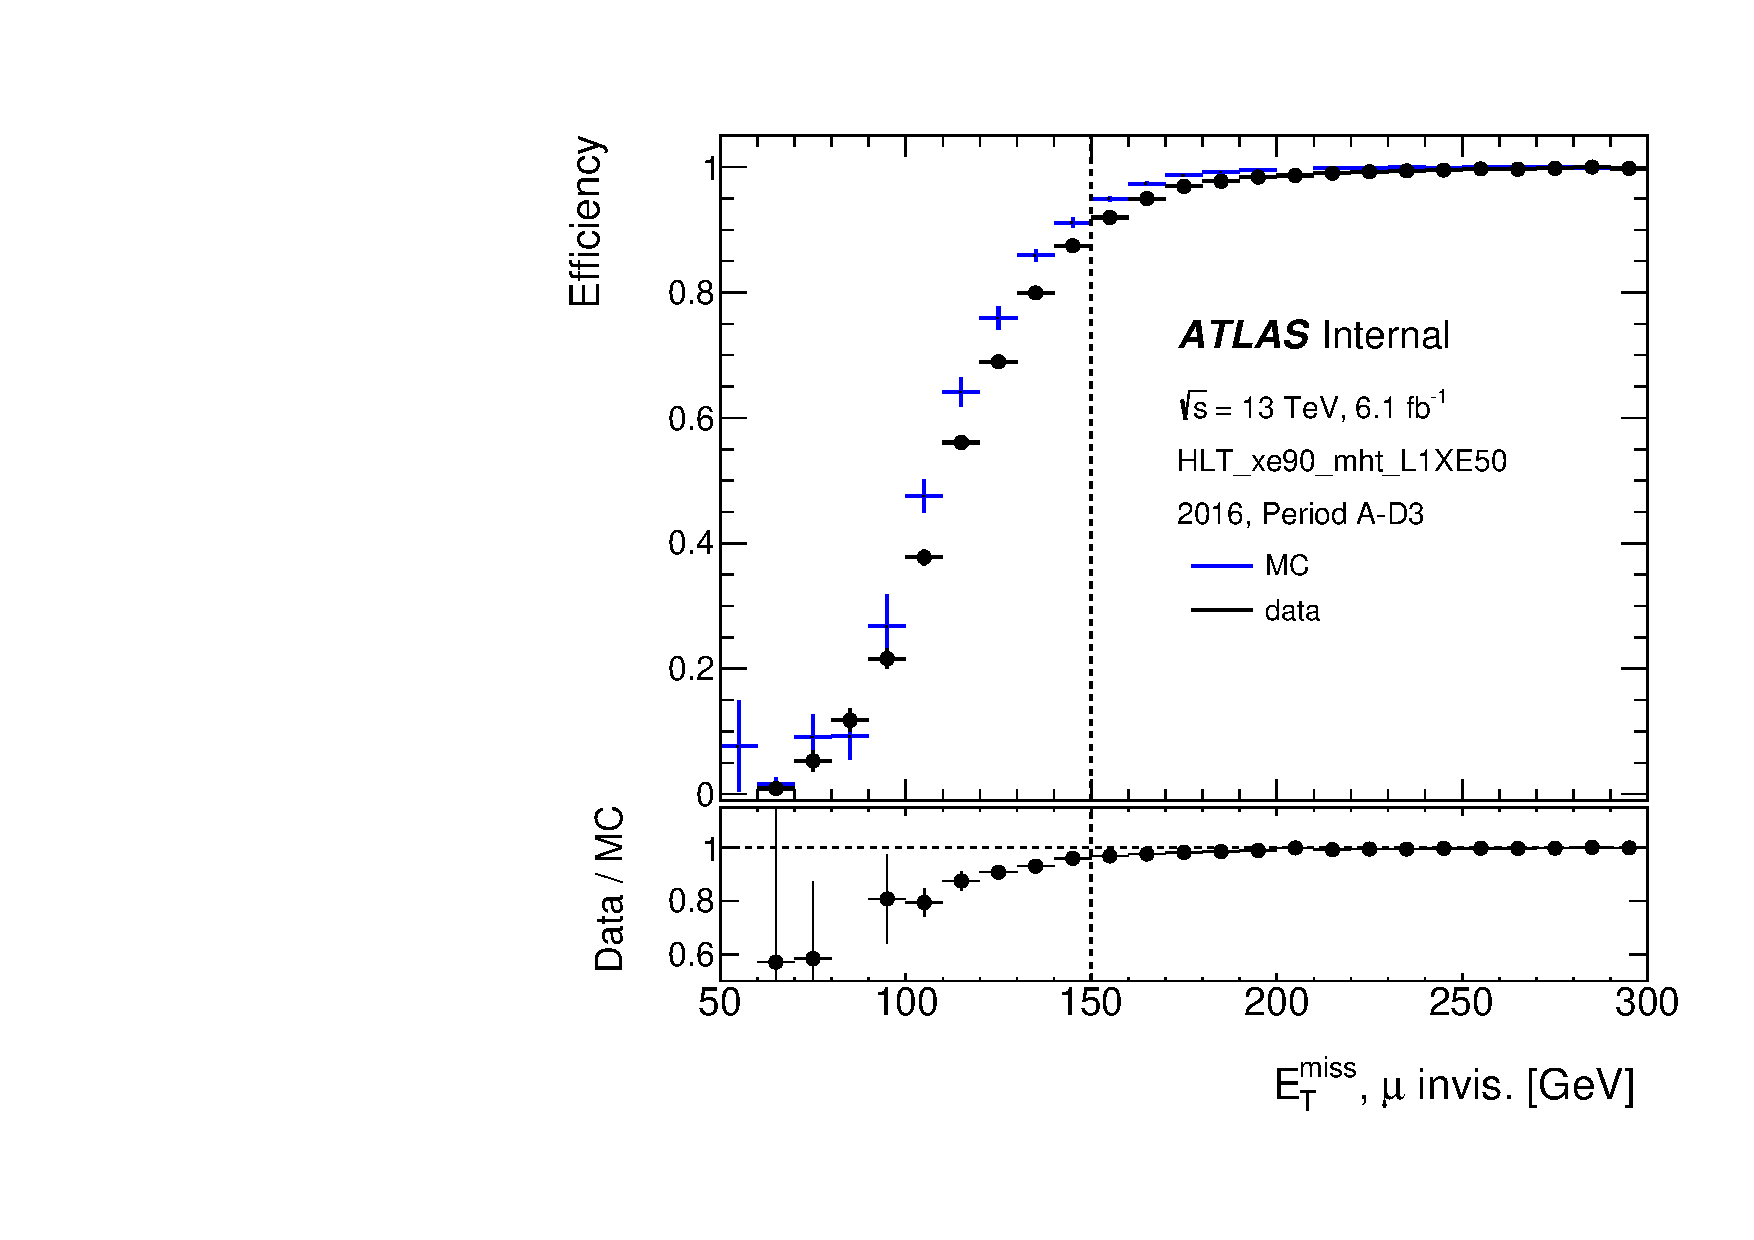
\includegraphics[width=0.45\textwidth]{chapters/c6/fig/METTriggerCalibration/efficiecy_HLT_xe90_mht_L1XE50.pdf}
	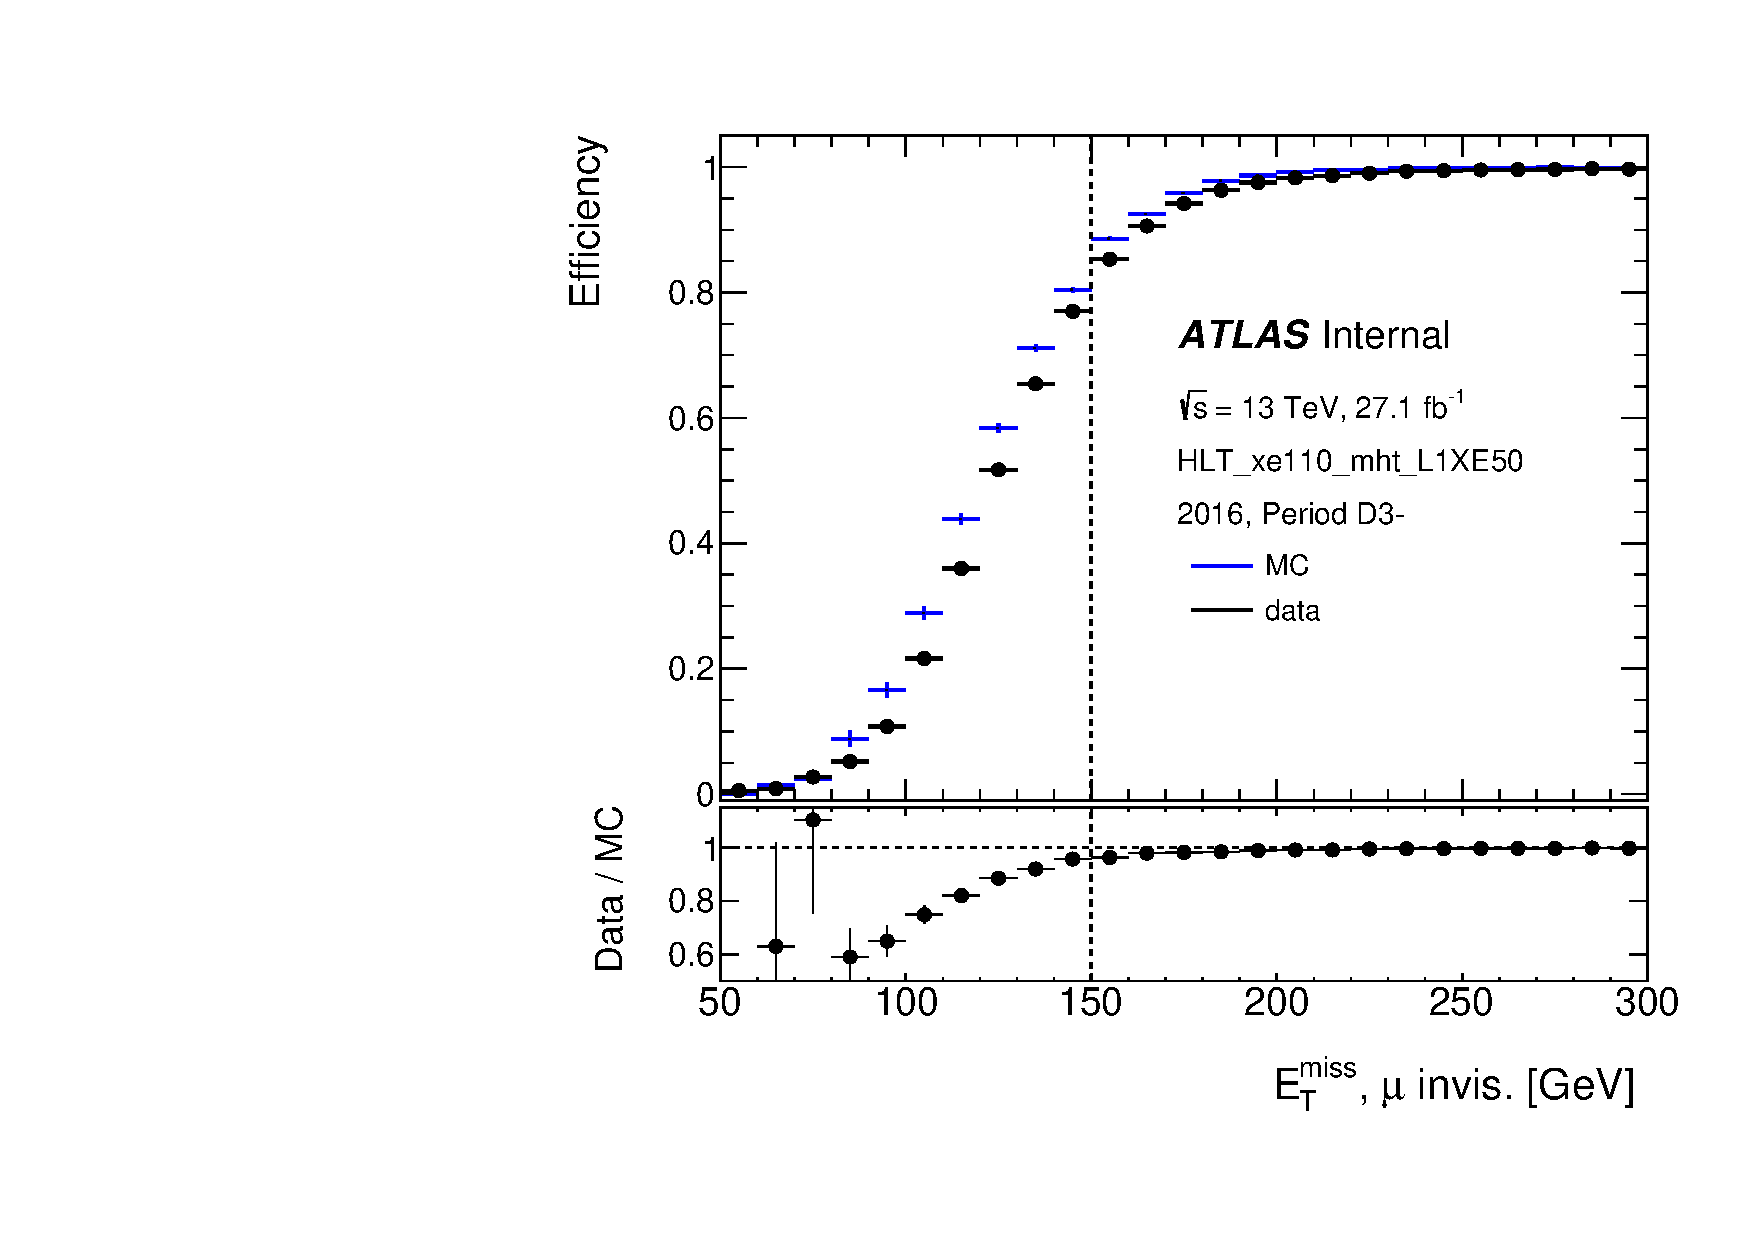
\includegraphics[width=0.45\textwidth]{chapters/c6/fig/METTriggerCalibration/efficiecy_HLT_xe110_mht_L1XE50.pdf}
	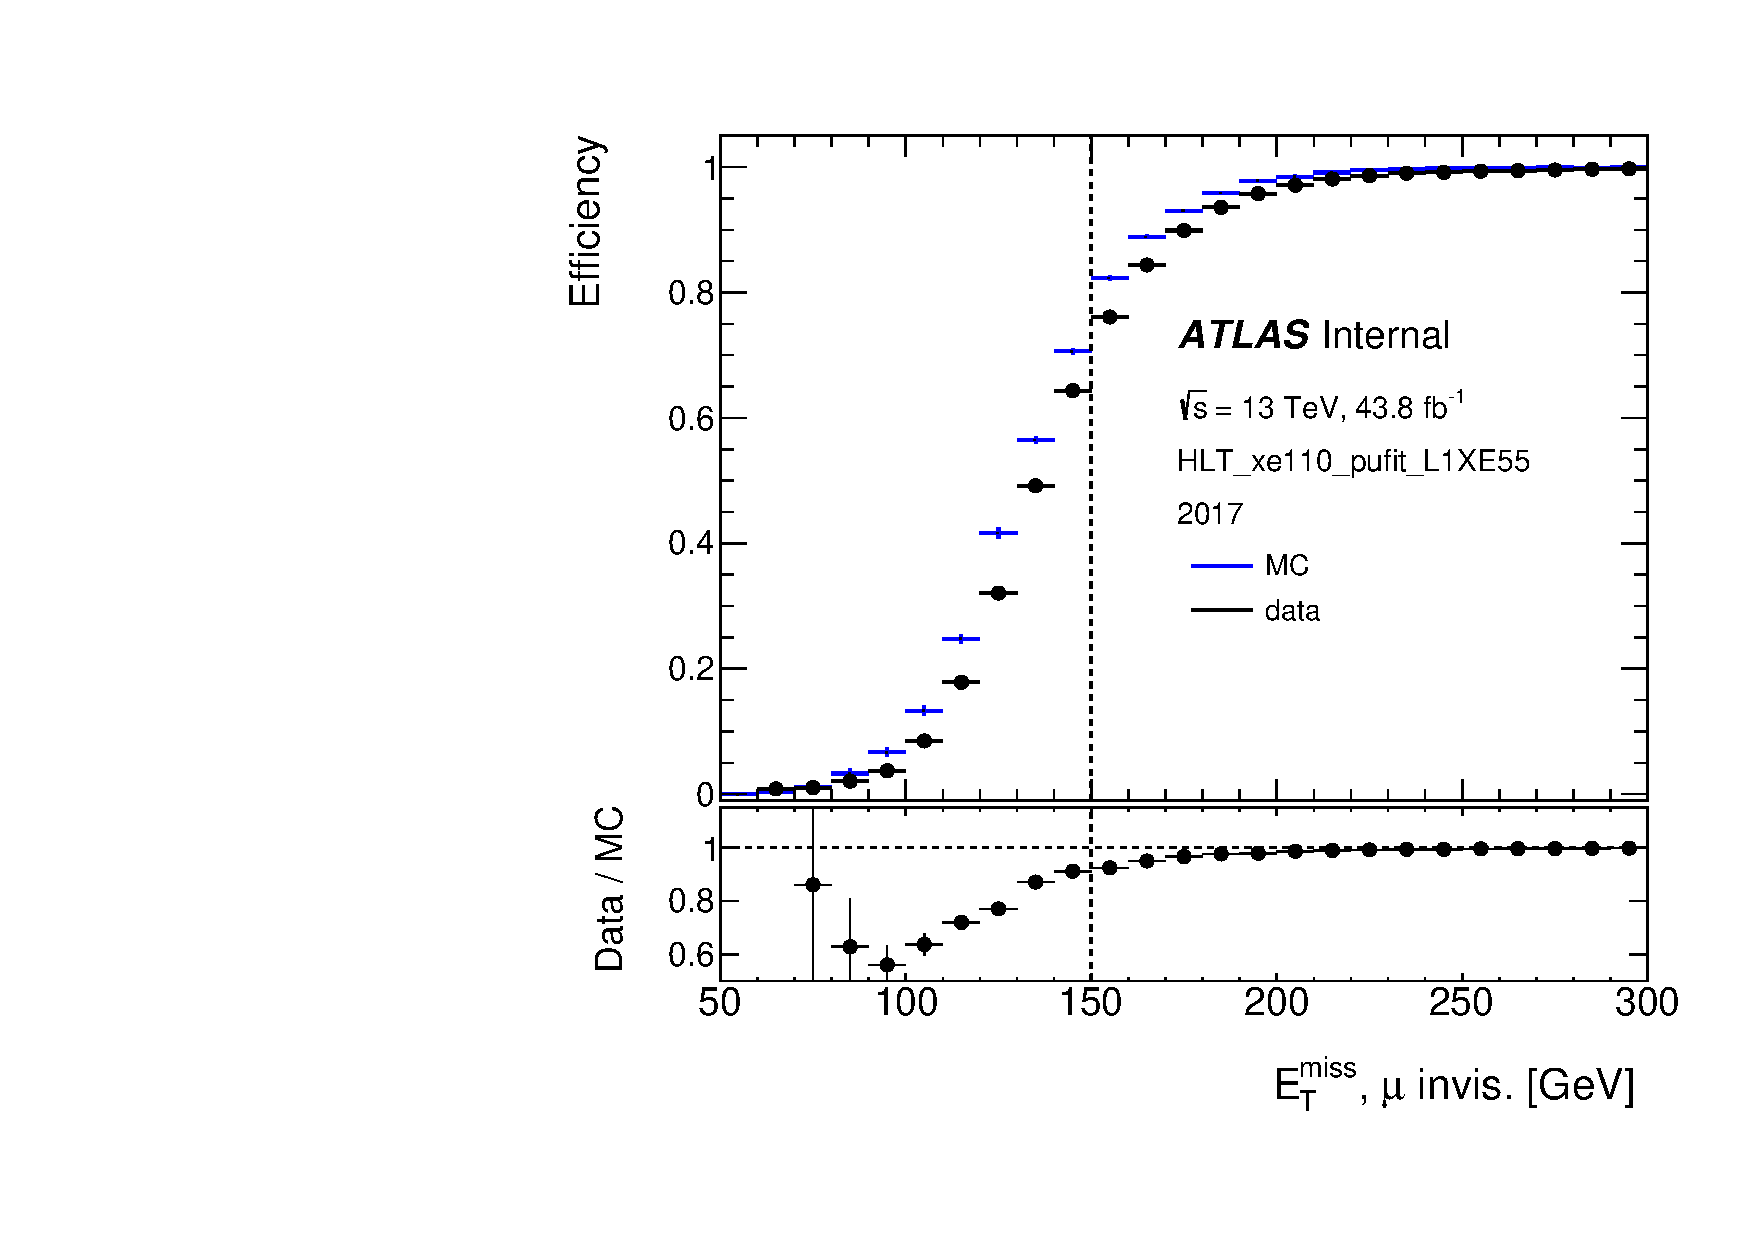
\includegraphics[width=0.45\textwidth]{chapters/c6/fig/METTriggerCalibration/efficiecy_HLT_xe110_pufit_L1XE55.pdf}
	\caption{Measured trigger efficiencies as a function of offline \METnomu~in data and MC for the \MET~triggers used in 2015-2018. The plots are shown for 0,1 and 2 tags together. The lower panels provide the ratio of data and MC events (the scale factor).}
	\label{fig:TrigEff}
\end{figure}
\par Scale factors (SF) are defined as the ratio of \MET~trigger efficiencies for data and MC:
\begin{equation}
\label{eq:dataMCsf}
\text{SF} = \frac{\text{Efficiency}^{\text{data}}_{\mu}}{\text{Efficiency}^{\text{MC}}_{\mu}}
\end{equation}
To calculate the data-driven corrections for the MC trigger turn-on curves, the scale factors are fitted for each \MET~trigger starting in the range $100~\GeV < \METnomu~< 300~\GeV$ in \MET~bins of 10~\GeV using the following fit function:
\begin{eqnarray}
\label{eq:dataMCsf_fit}
f\left(\text{x}\right) = p_0 \cdot \left[1 + \text{erf}\left(\frac{\text{x} - p_{1}}{\sqrt{2}p_{2}}\right)\right] + p_3
\end{eqnarray}

where $x = \METnomu$.
\par The scale factor applied to the MC in the signal region and one-lepton control region is given by evaluating $f(\met)$ or $f(\METnomu)$,
 respectively. The scale factors measured for the different \MET~are shown in Fig.~\ref{fig:TrigSF} together with the fitted SF curves.
 Good agreement is observed in data and MC efficiencies comparison in Figure~\ref{fig:TrigSF_validation}, after the scale factors are applied to the simulation.


\begin{figure}[tb!]
	\centering
	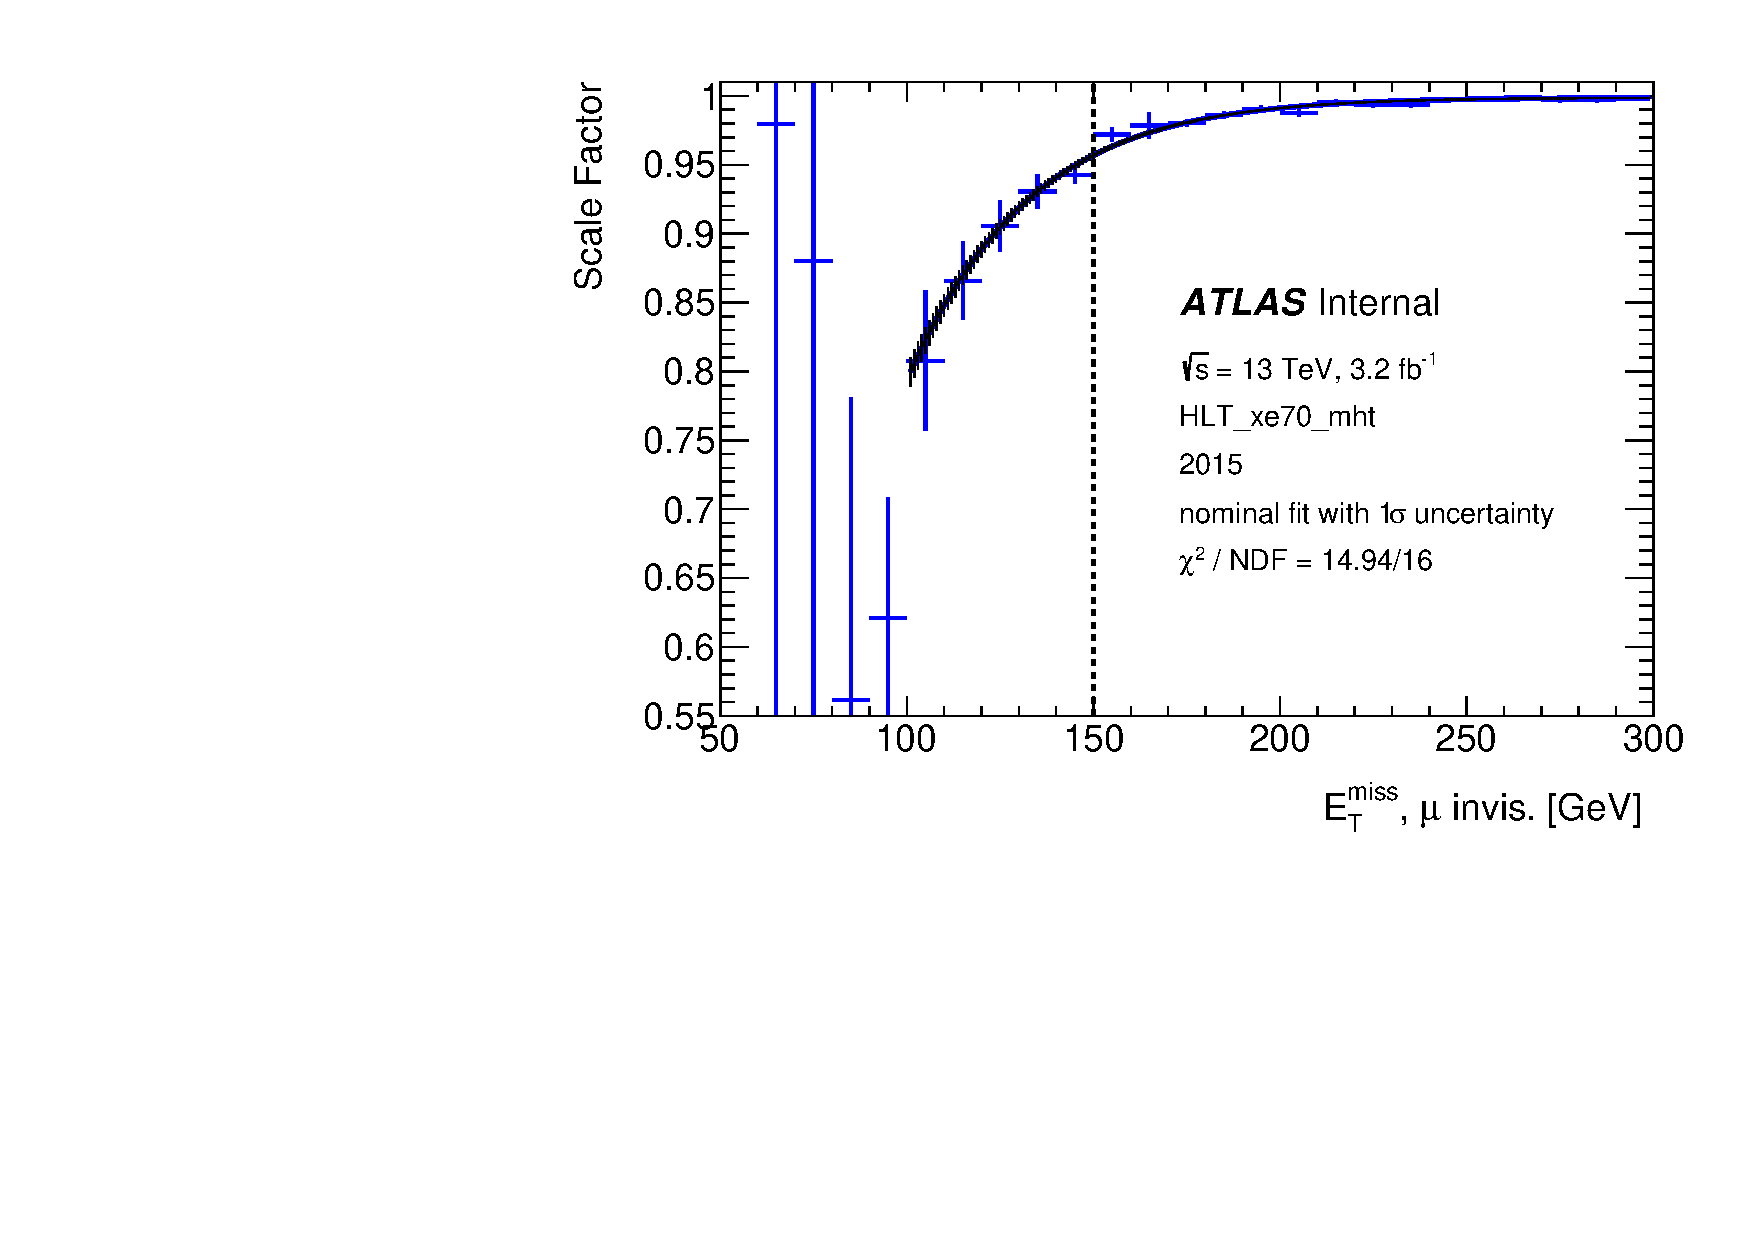
\includegraphics[width=0.45\textwidth]{chapters/c6/fig/METTriggerCalibration/SF_HLT_xe70_mht.pdf}
	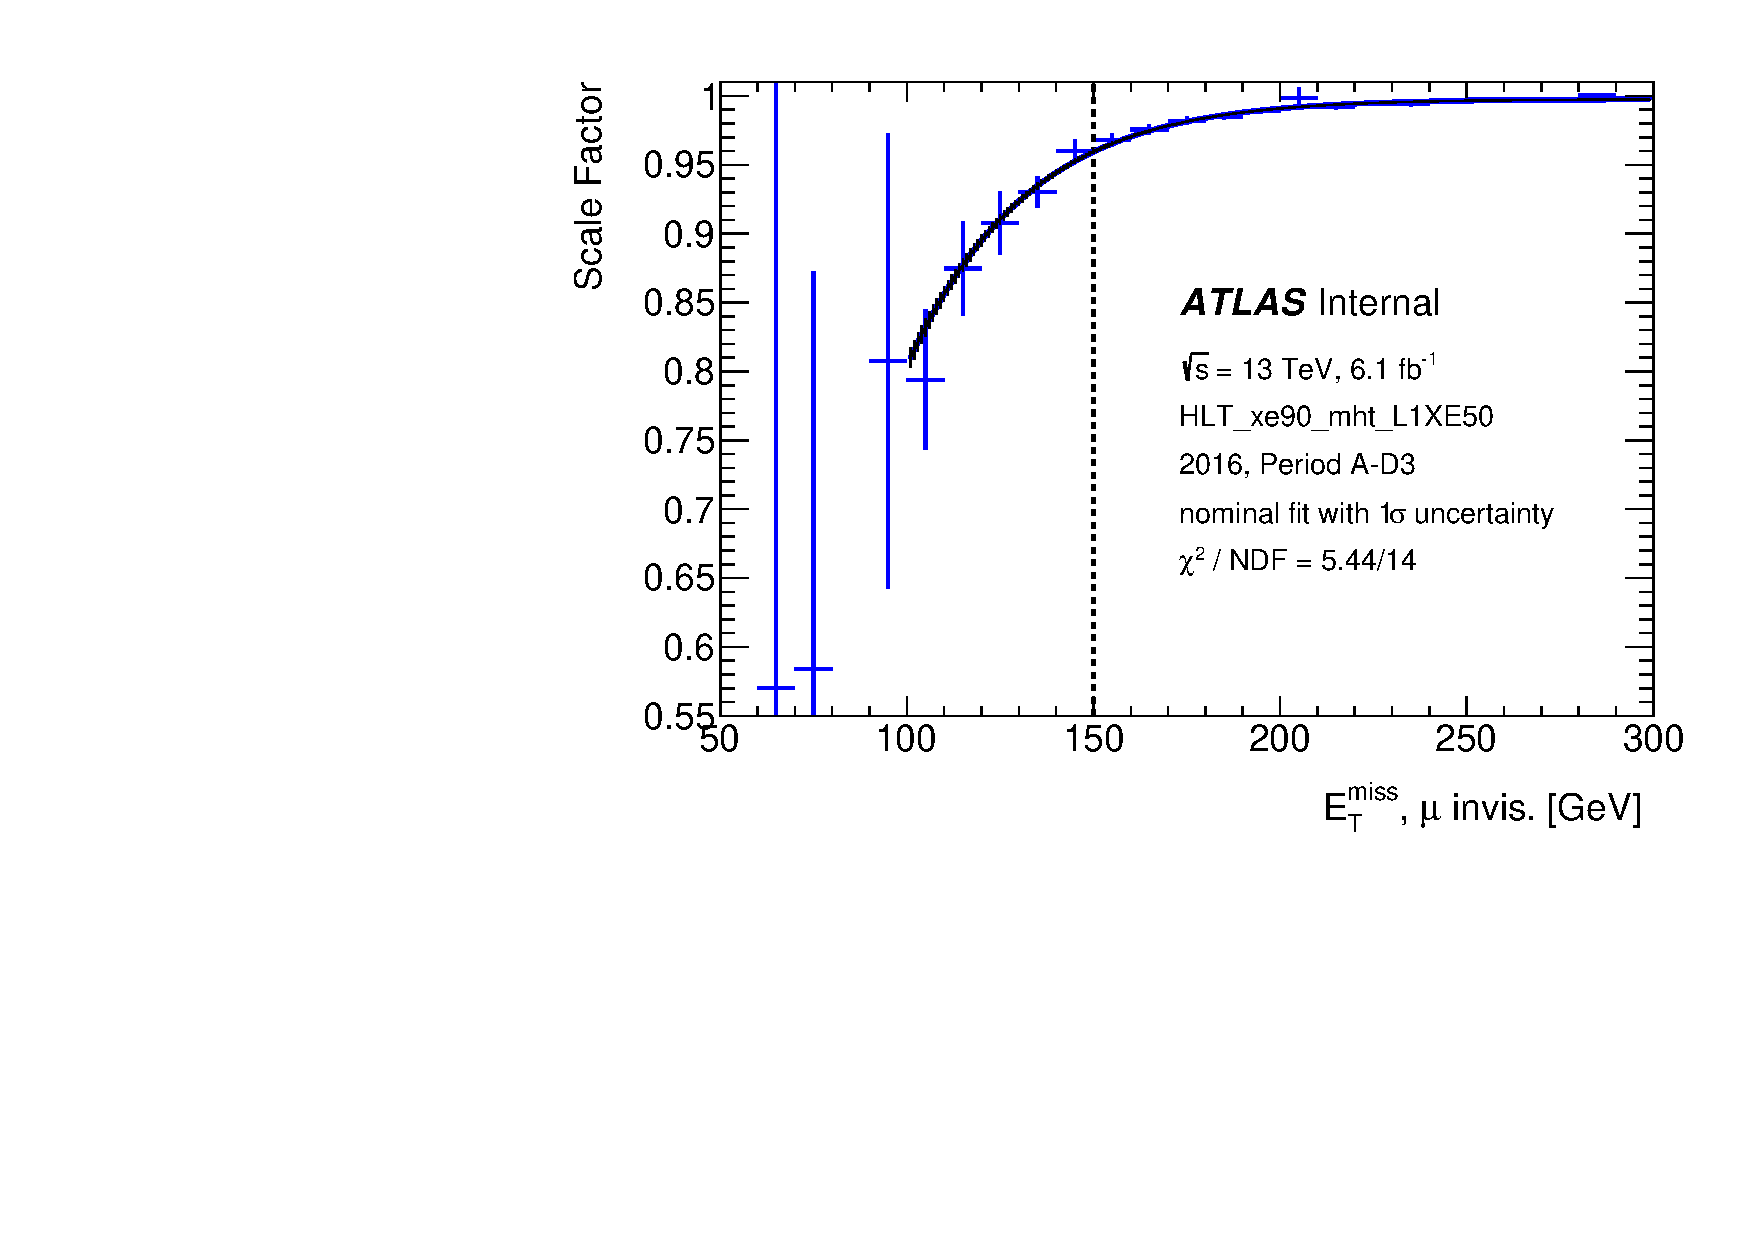
\includegraphics[width=0.45\textwidth]{chapters/c6/fig/METTriggerCalibration/SF_HLT_xe90_mht_L1XE50.pdf}
	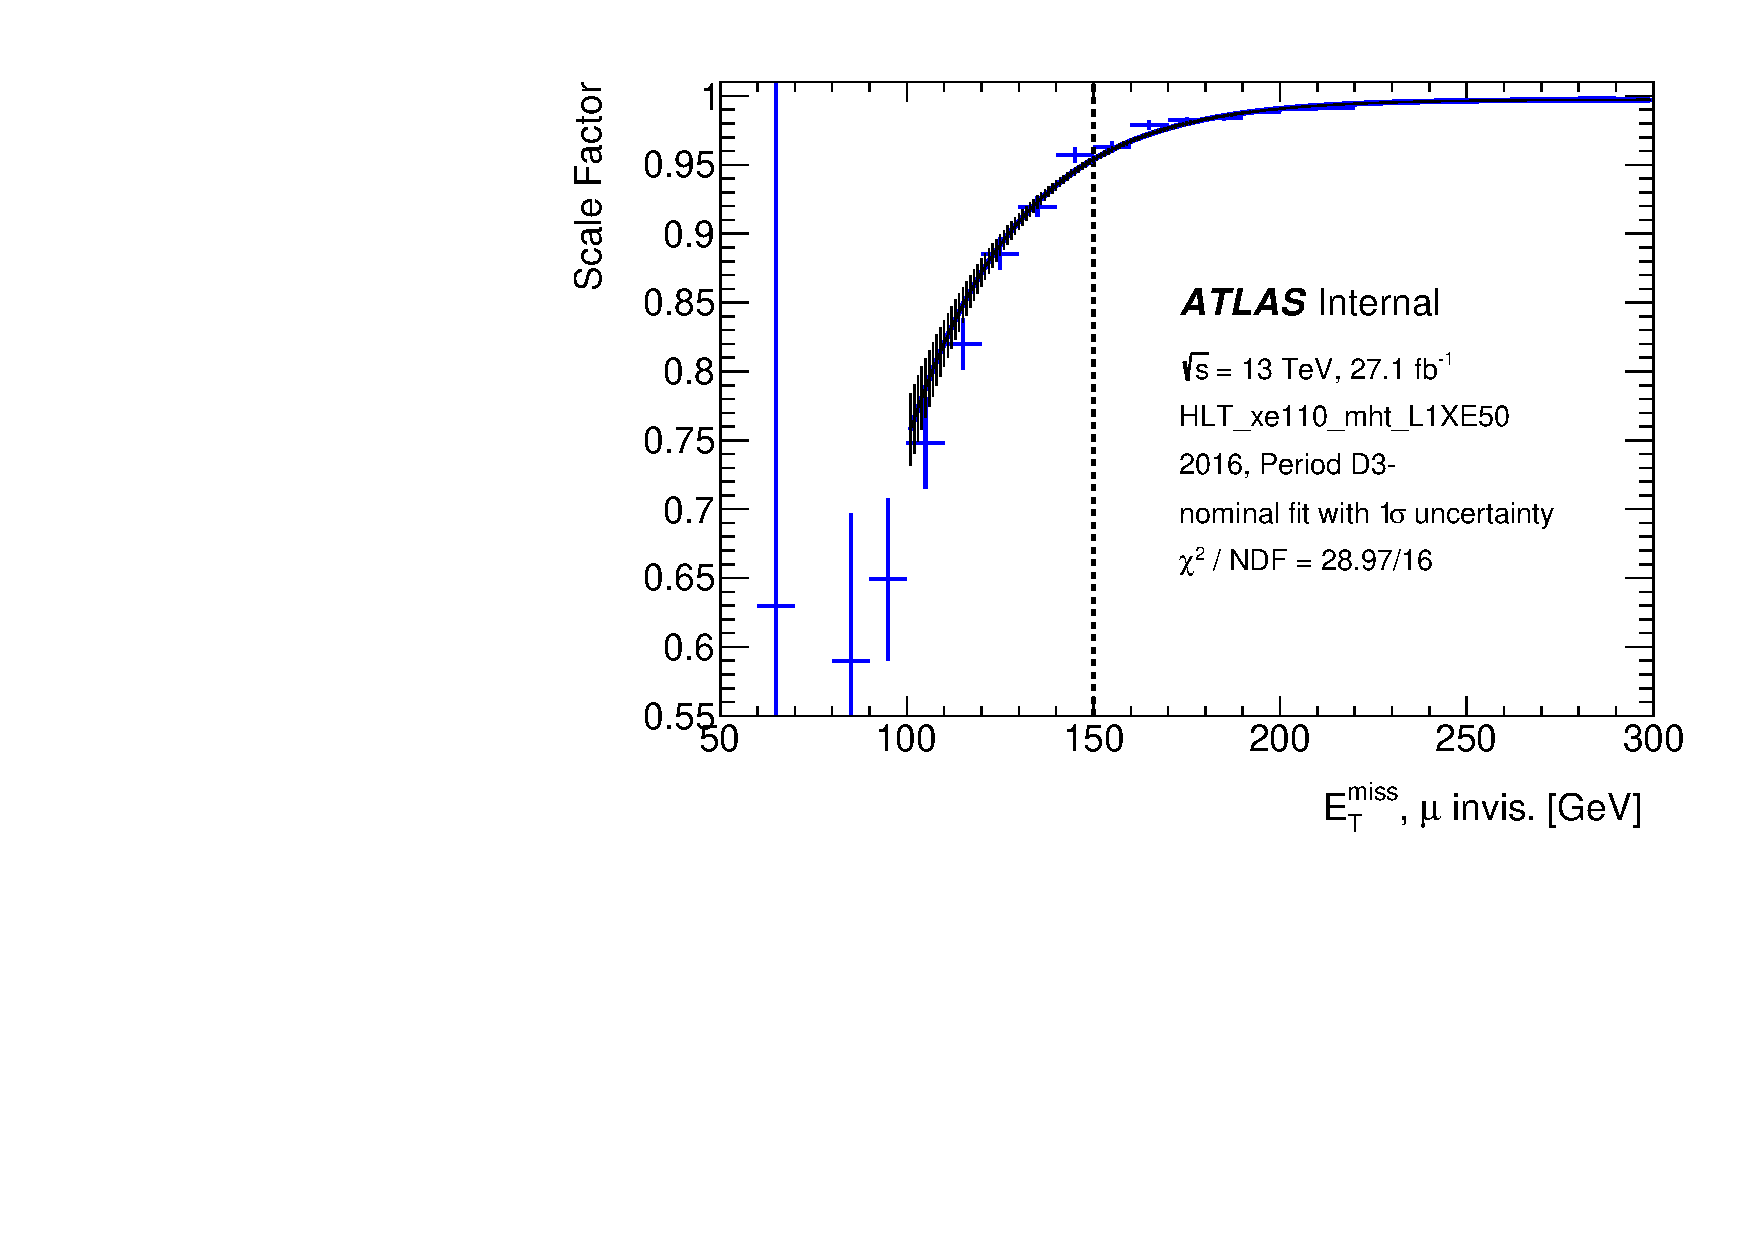
\includegraphics[width=0.45\textwidth]{chapters/c6/fig/METTriggerCalibration/SF_HLT_xe110_mht_L1XE50.pdf}
	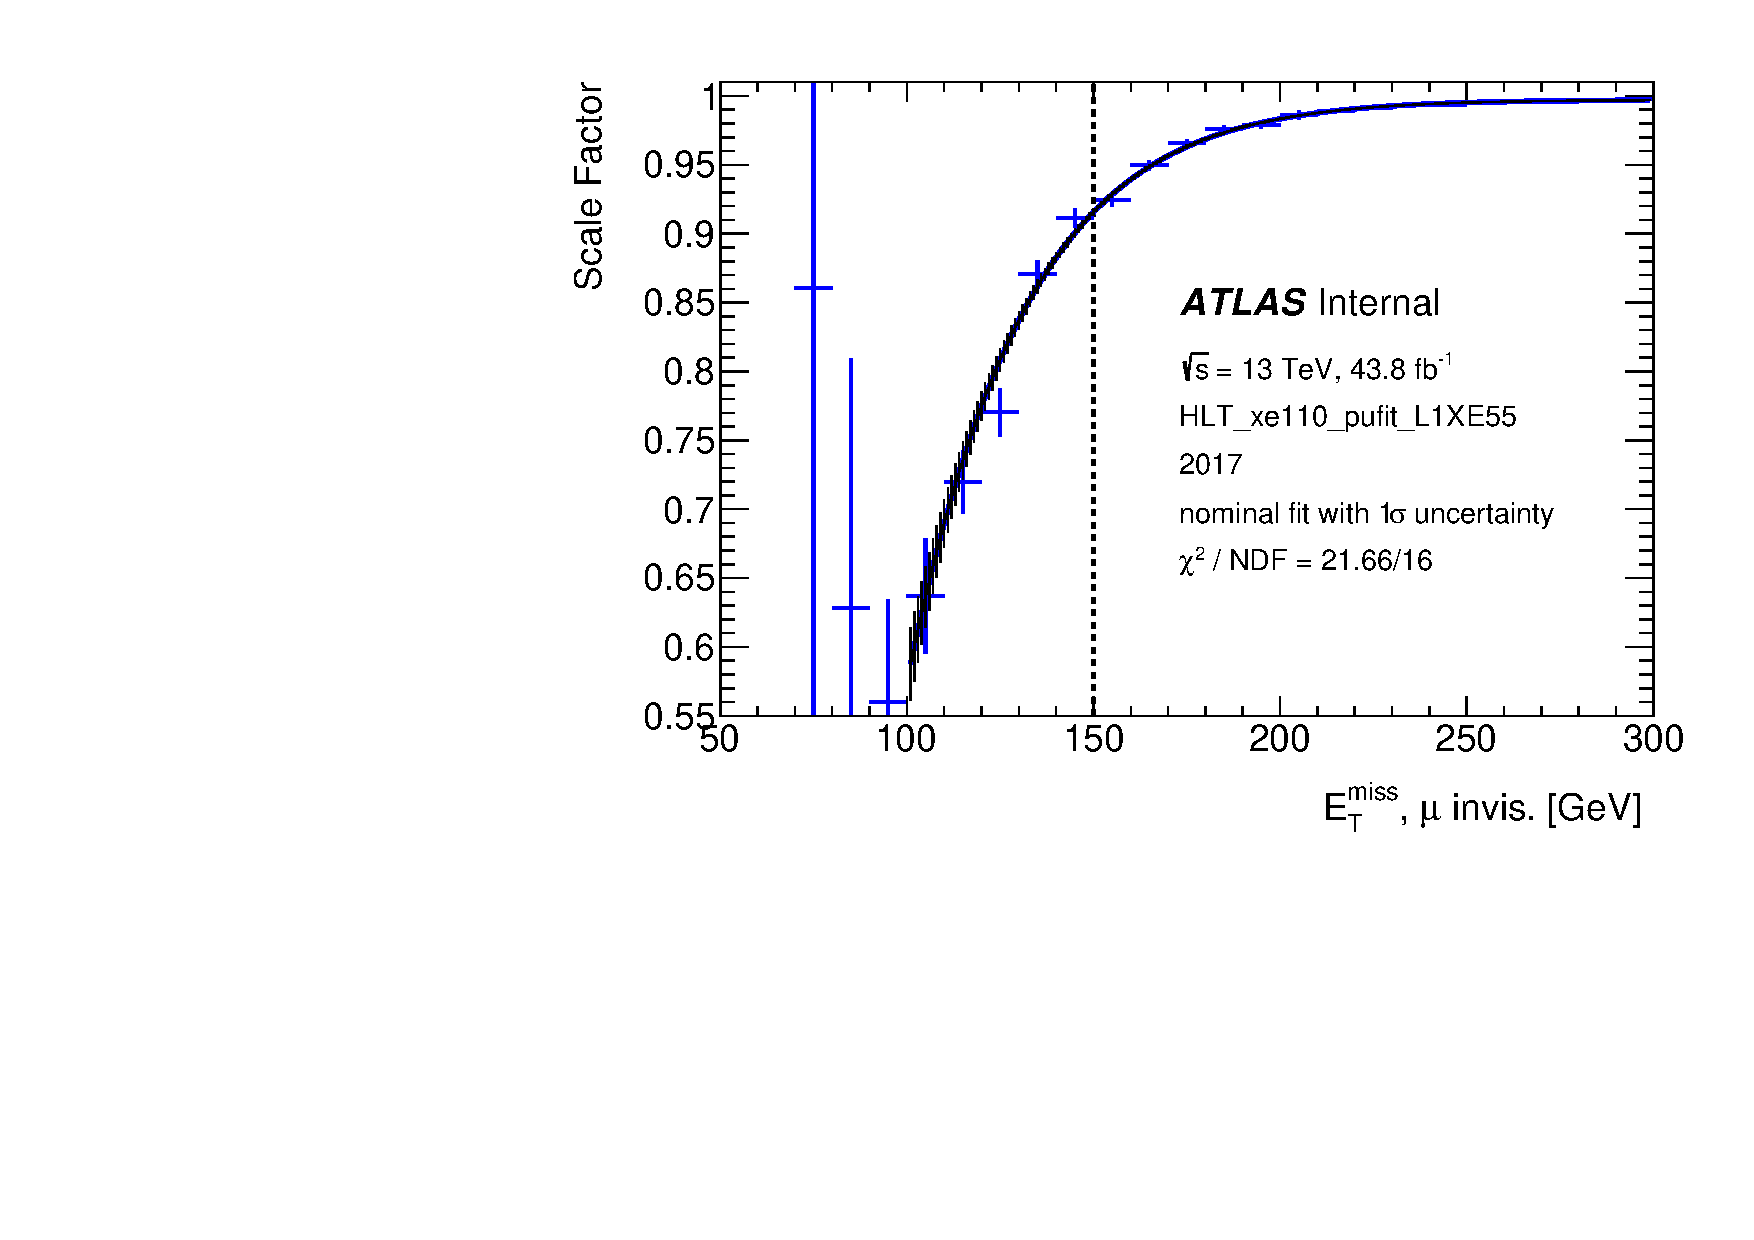
\includegraphics[width=0.45\textwidth]{chapters/c6/fig/METTriggerCalibration/SF_HLT_xe110_pufit_L1XE55.pdf}
	\caption{Measured scale factors as a function of offline \METnomu~for the \MET~triggers used in 2015-2010. The scale factors were derived for 0,1 and 2 tags together. The hatched band shows the 1$\sigma$ fit uncertainty.}
	\label{fig:TrigSF}
\end{figure}

\begin{figure}[tb!]
	\centering
	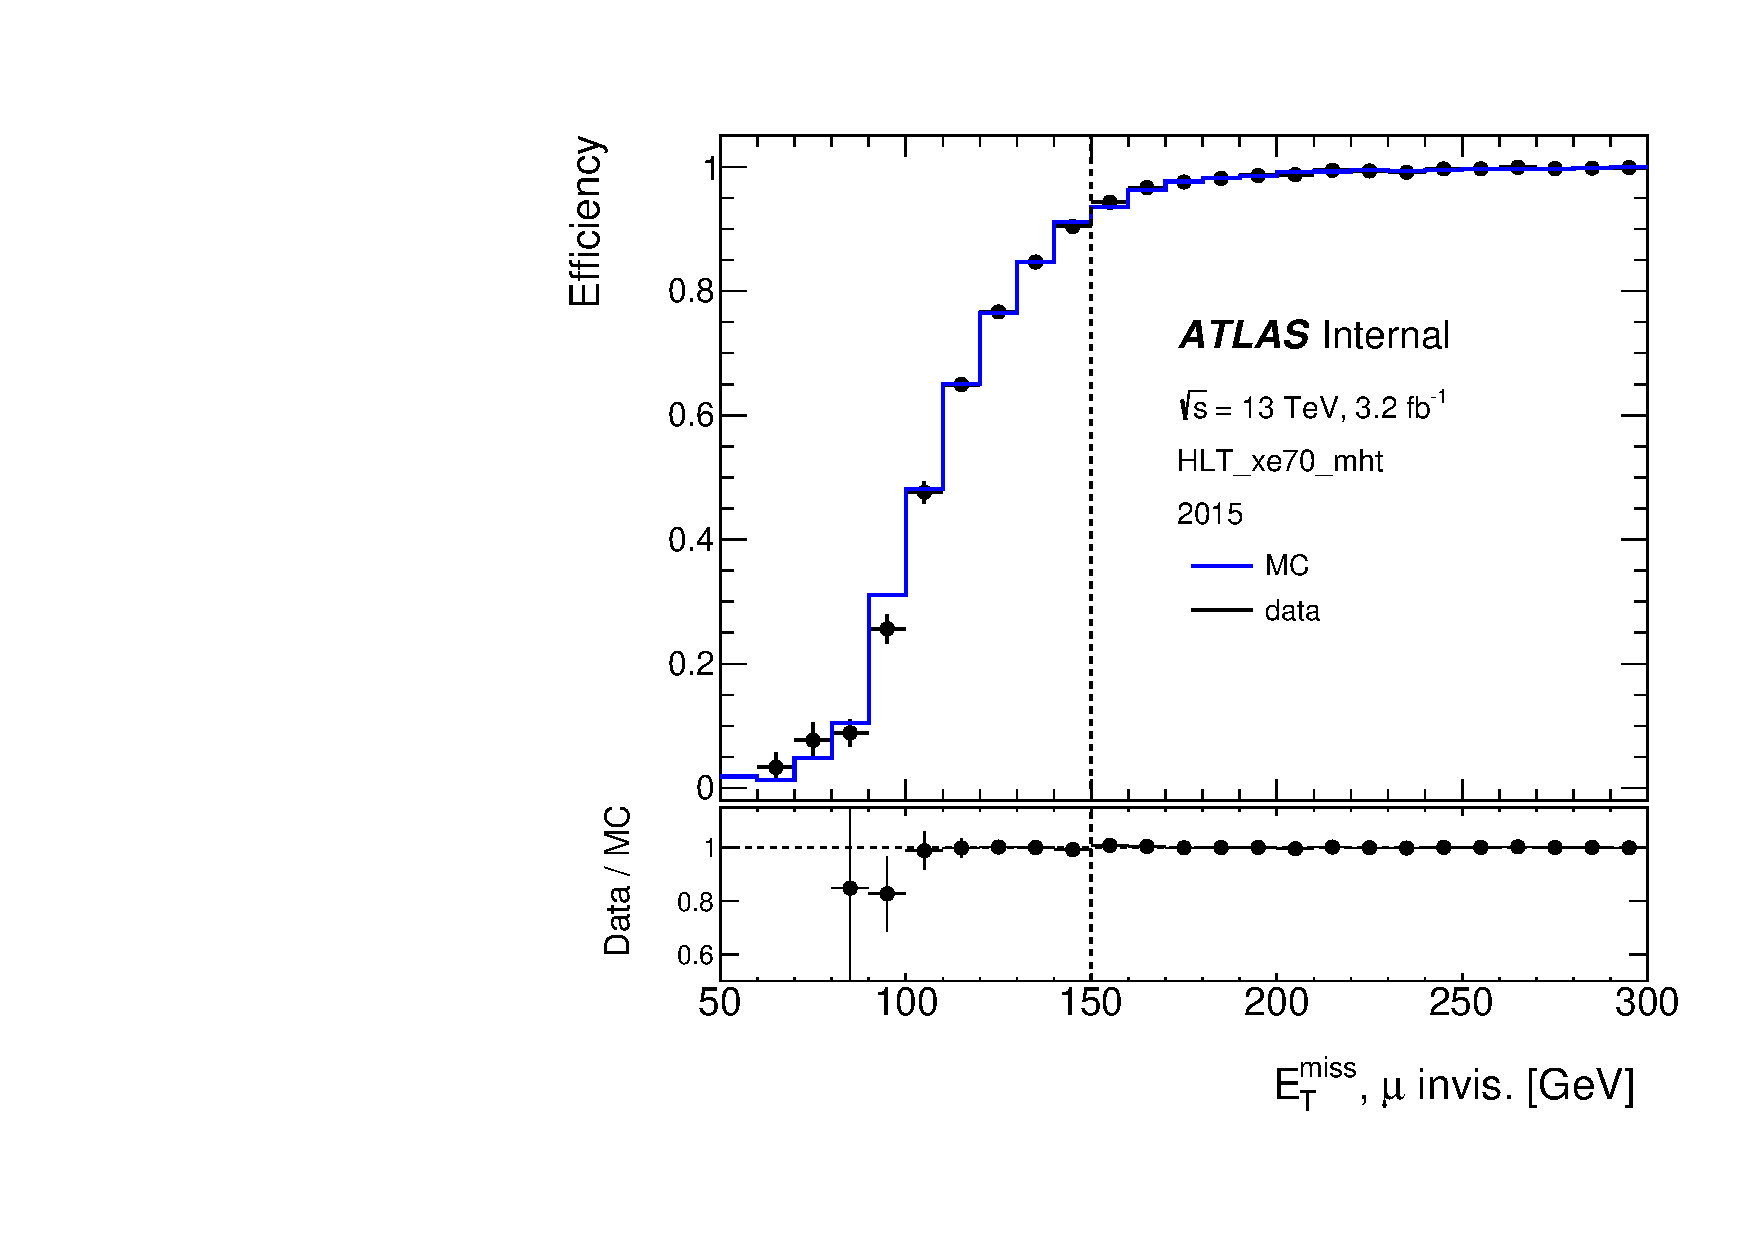
\includegraphics[width=0.45\textwidth]{chapters/c6/fig/METTriggerCalibration/validation_HLT_xe70_mht.pdf}
	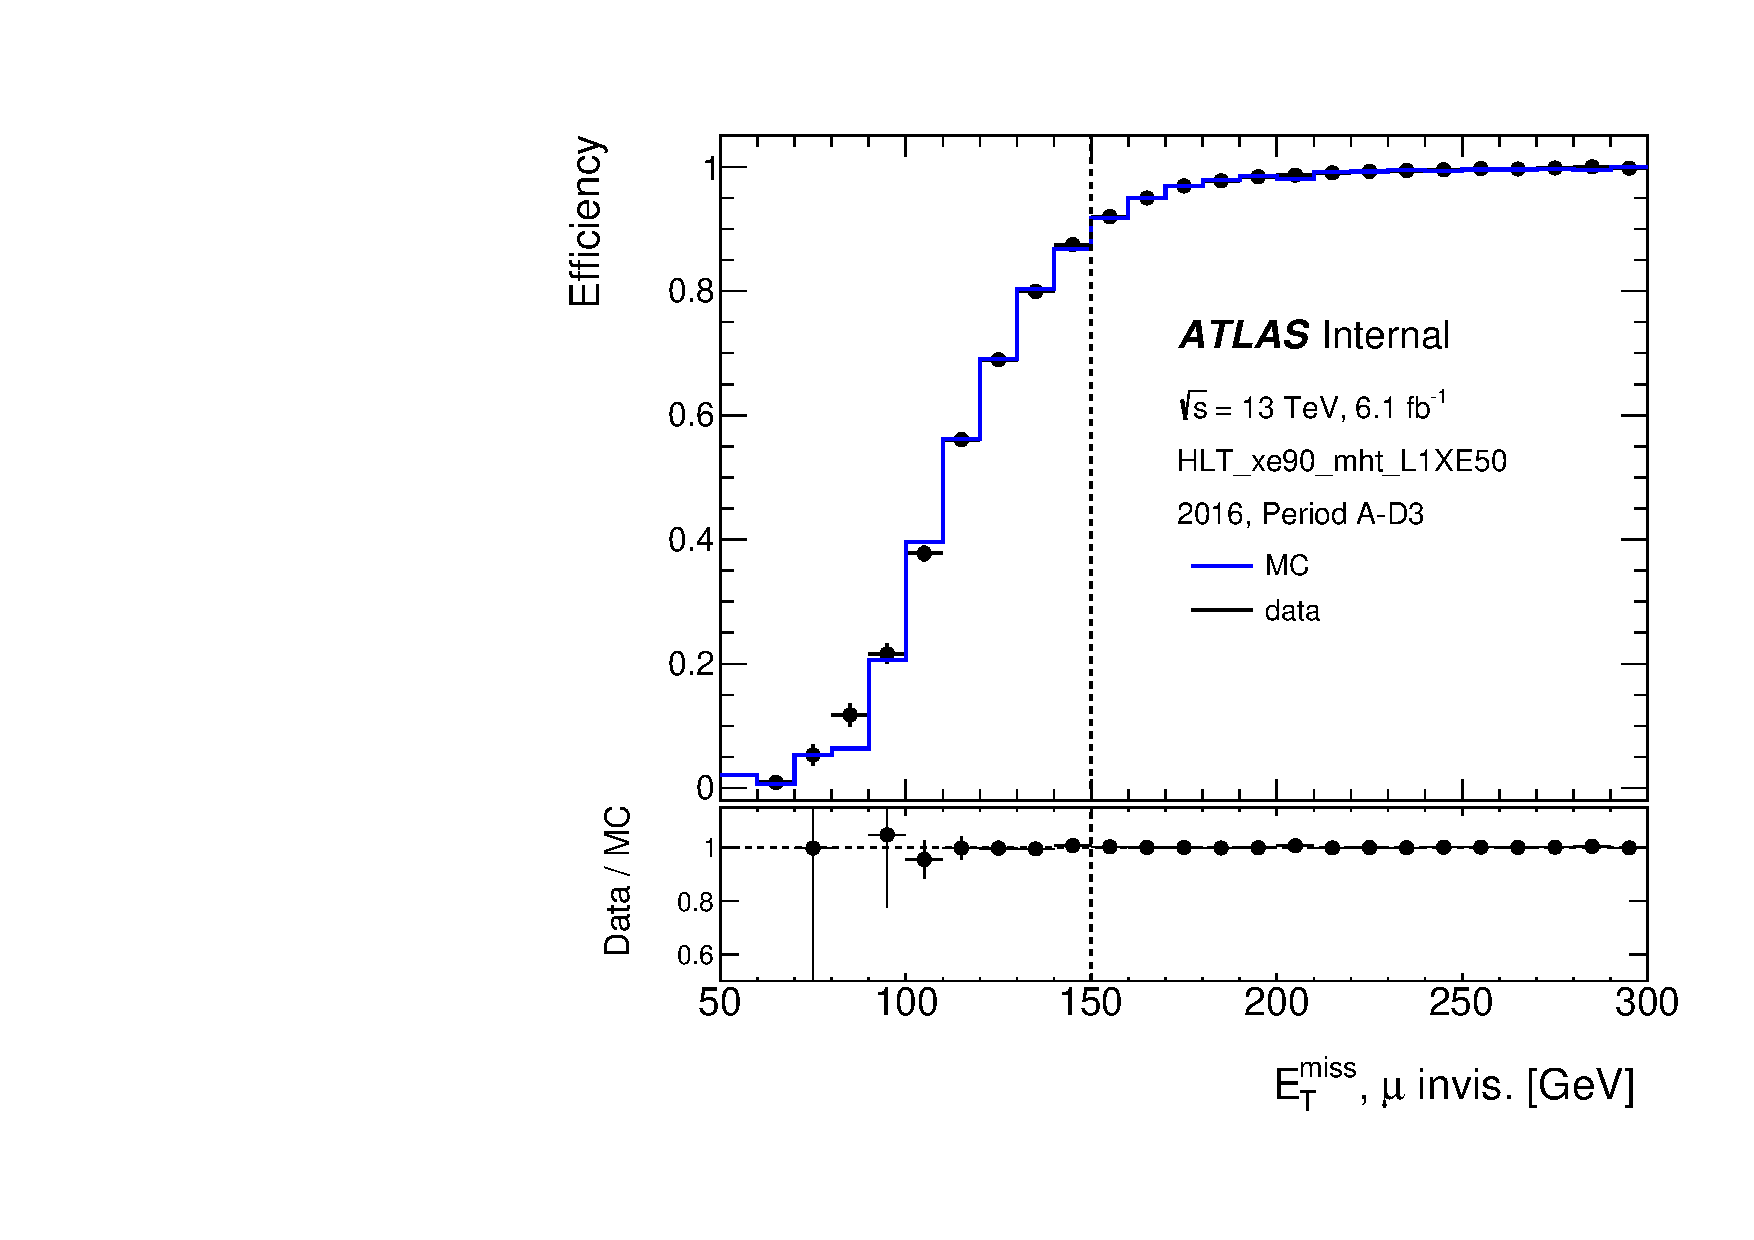
\includegraphics[width=0.45\textwidth]{chapters/c6/fig/METTriggerCalibration/validation_HLT_xe90_mht_L1XE50.pdf}
	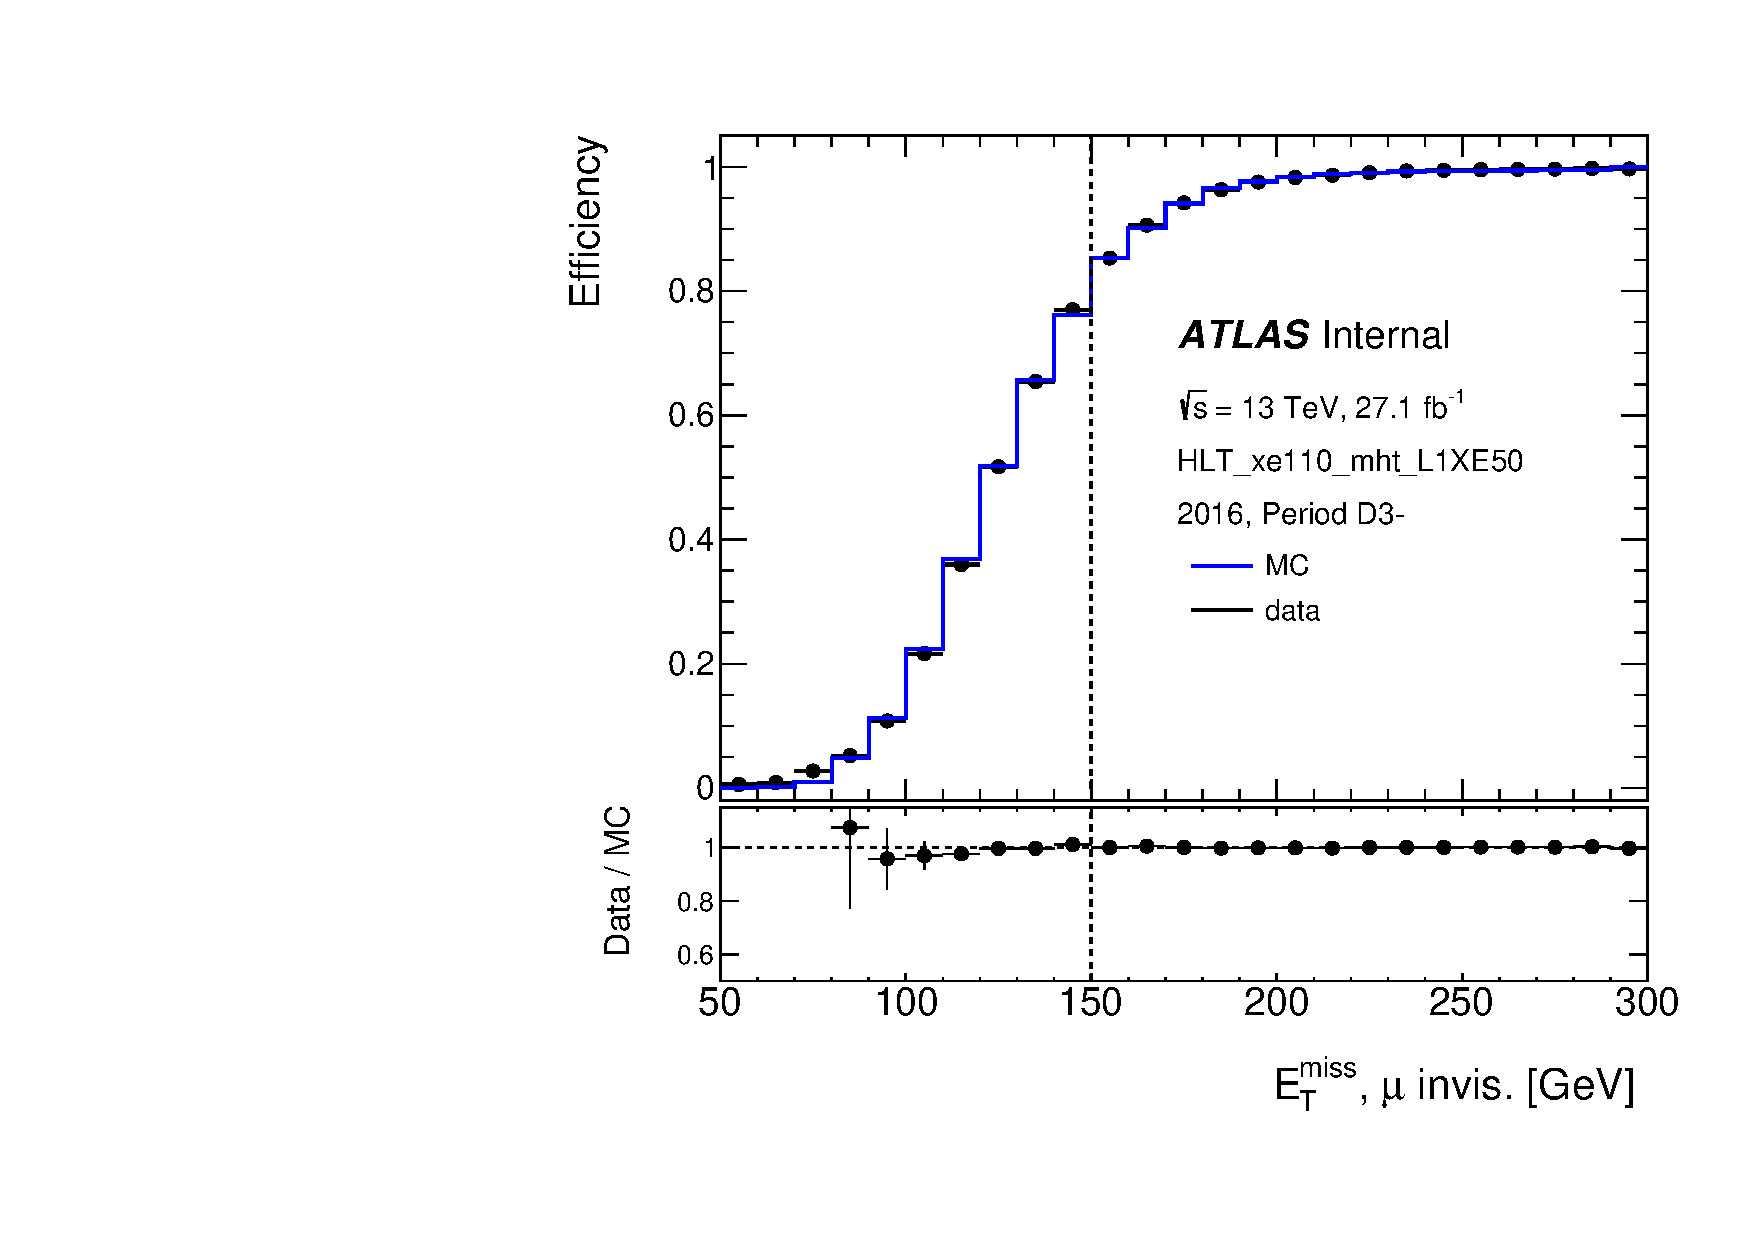
\includegraphics[width=0.45\textwidth]{chapters/c6/fig/METTriggerCalibration/validation_HLT_xe110_mht_L1XE50.pdf}
	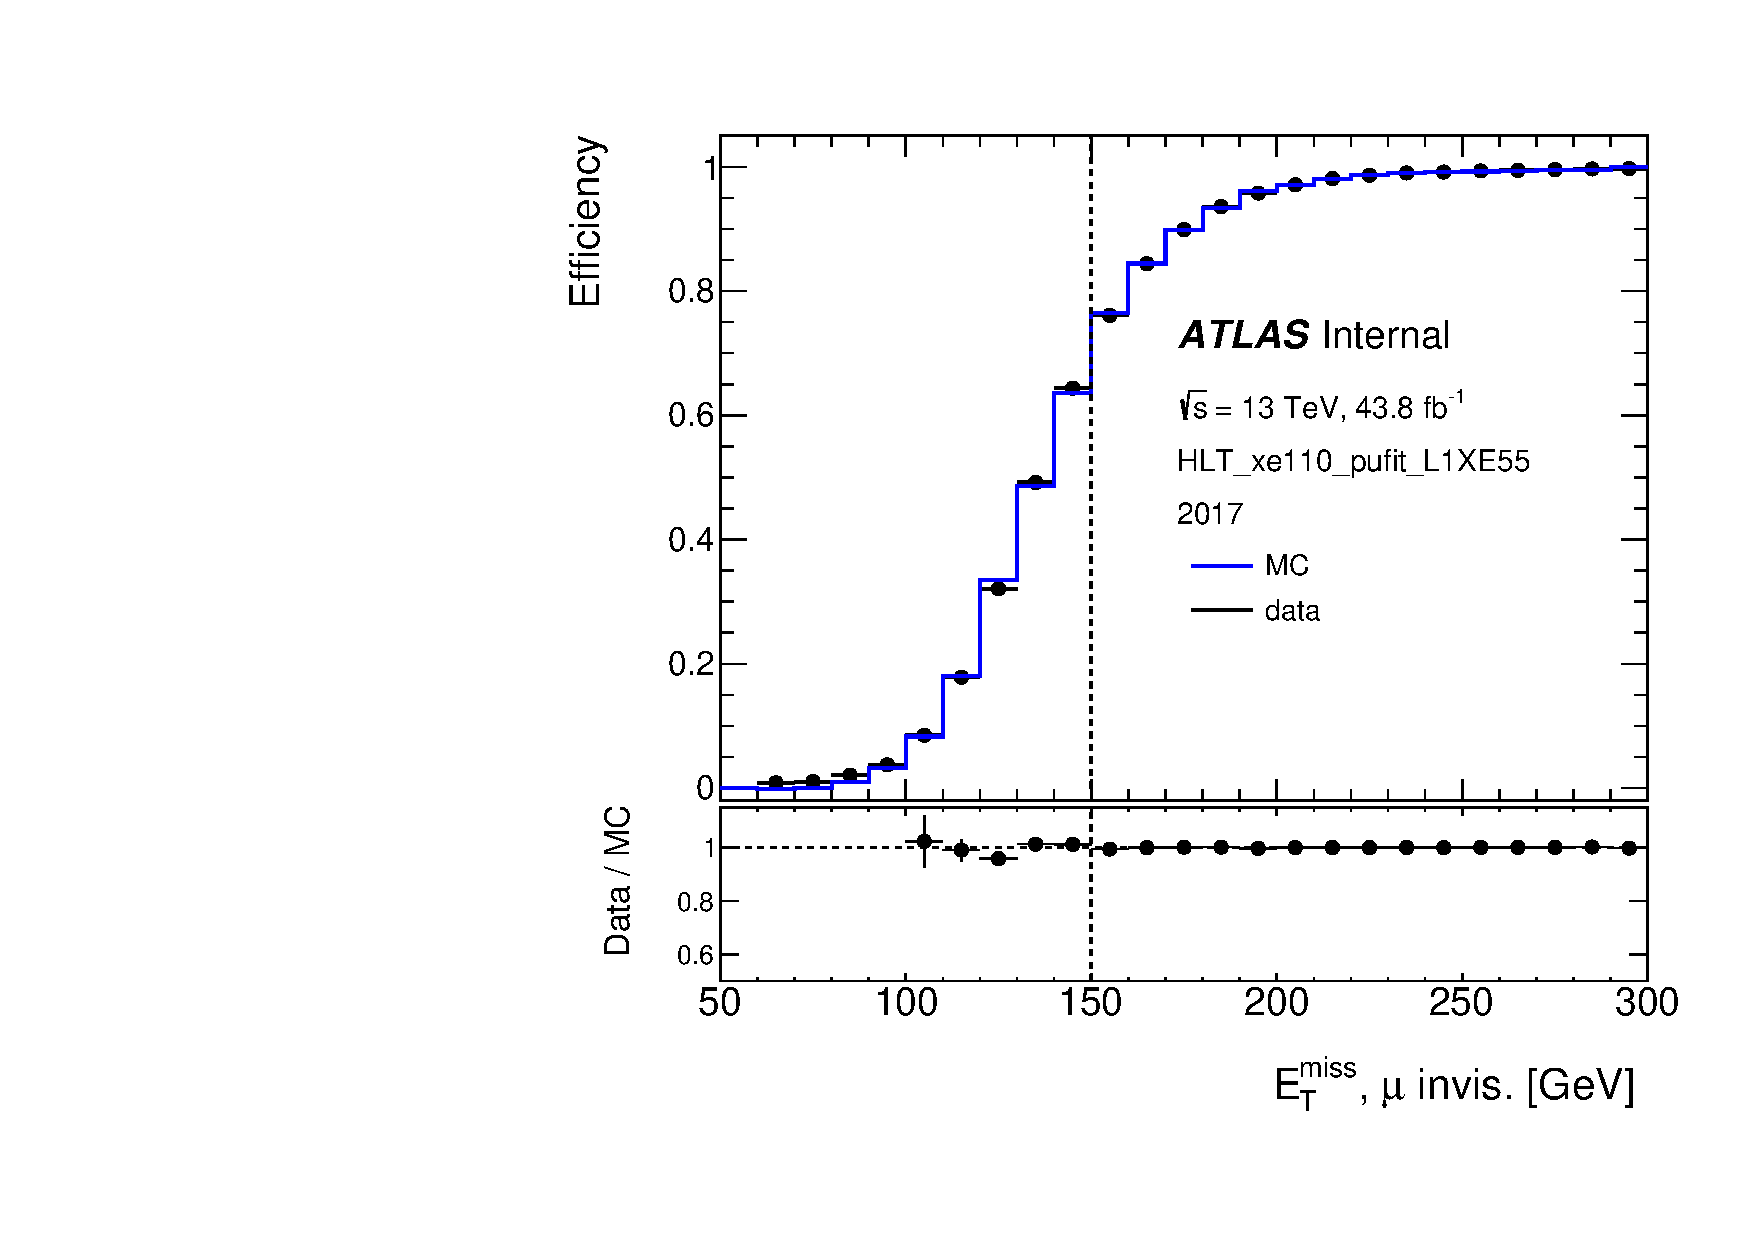
\includegraphics[width=0.45\textwidth]{chapters/c6/fig/METTriggerCalibration/validation_HLT_xe110_pufit_L1XE55.pdf}
	\caption{Validation plots showing \MET~trigger efficiencies and scale factors as function of offline \METnomu~after applying scale factor corrections for $\METnomu>100\,\GeV$ to the MC in the full single lepton region. Good agreement is observed between data and MC.}
	\label{fig:TrigSF_validation}
\end{figure}


\par The triggers are listed in Table~\ref{tab:summary_triggers_used}. 

\begin{table}
	\scriptsize{
		\begin{center}

			\resizebox{1.\textwidth}{!}{
				\begin{tabular}{ c c c c}
					\hline
					\hline
					Period & 0 lepton & 1 lepton & 2 lepton + \met~trigger SF measurement \\
					\hline
					2015 & \textsc{HLT\_xe70\_mht} & \textsc{HLT\_xe70\_mht} & \textsc{HLT\_e24\_lhmedium\_L1EM20VH}\\
					& & & \textbf{OR} \textsc{HLT\_e120\_lhloose}  \\ 
					& & & \textbf{OR} \textsc{HLT\_mu20\_iloose\_L1MU15} \\
					& & & \textbf{OR} \textsc{HLT\_mu50} \\
					\hline
					2016 & \textsc{HLT\_xe90\_mht\_L1XE50} & \textsc{HLT\_xe90\_mht\_L1XE50} & \textsc{HLT\_e60\_lhmedium\_nod0}  \\
					(A) & & & \textbf{OR} \textsc{HLT\_e140\_lhloose\_nod0} \\ 
					& & & \textbf{OR} \textsc{HLT\_mu40} \\
					& & & \textbf{OR} \textsc{HLT\_mu50} \\
					\hline
					2016 & \textsc{HLT\_xe90\_mht\_L1XE50} & \textsc{HLT\_xe90\_mht\_L1XE50} & \\
                    (B-D3) & & & \textsc{HLT\_e60\_lhmedium\_nod0} \\
					& & & \textbf{OR} \textsc{HLT\_e140\_lhloose\_nod0} \\ 
					& & & \textbf{OR} \textsc{HLT\_mu24\_ivarmedium} \\
					& & & \textbf{OR} \textsc{HLT\_mu50} \\
					\hline
					2016 & \textsc{HLT\_xe110\_mht\_L1XE50} & \textsc{HLT\_xe110\_mht\_L1XE50} & \textsc{HLT\_e26\_lhtight\_nod0\_ivarloose} \\	
					(D4-E3)& & & \textbf{OR} \textsc{HLT\_e60\_lhmedium\_nod0} \\
					& & & \textbf{OR} \textsc{HLT\_e140\_lhloose\_nod0} \\ 
					& & & \textbf{OR} \textsc{HLT\_mu24\_ivarmedium} \\
					& & & \textbf{OR} \textsc{HLT\_mu26\_ivarmedium} \\
					& & & \textbf{OR} \textsc{HLT\_mu50} \\
					\hline
					2016 & \textsc{HLT\_xe110\_mht\_L1XE50} & \textsc{HLT\_xe110\_mht\_L1XE50} & \textsc{HLT\_e26\_lhtight\_nod0\_ivarloose}\\
                    (F1)&  & & \textbf{OR} \textsc{HLT\_e60\_lhmedium\_nod0} \\
					& & & \textbf{OR} \textsc{HLT\_e140\_lhloose\_nod0} \\ 
					& & & \textbf{OR} \textsc{HLT\_mu26\_ivarmedium} \\
					& & & \textbf{OR} \textsc{HLT\_mu50} \\
					\hline
					2016 & \textsc{HLT\_xe110\_mht\_L1XE50} & \textsc{HLT\_xe110\_mht\_L1XE50} &\textsc{HLT\_e26\_lhtight\_nod0\_ivarloose} \\
					(F2-) & & & \textbf{OR} \textsc{HLT\_e60\_lhmedium\_nod0} \\
					& & & \textbf{OR} \textsc{HLT\_e140\_lhloose\_nod0} \\ 
					& & & \textbf{OR} \textsc{HLT\_mu26\_ivarmedium} \\
					& & & \textbf{OR} \textsc{HLT\_mu50} \\
					\hline
					2017 & \textsc{HLT\_xe110\_pufit\_L1XE55} & \textsc{HLT\_xe110\_pufit\_L1XE55} &\textsc{HLT\_e60\_lhmedium\_nod0} \\
					& & & \textbf{OR} \textsc{HLT\_e140\_lhloose\_nod0} \\
					& & & \textbf{OR} \textsc{HLT\_mu26\_ivarmedium} \\
					& & & \textbf{OR} \textsc{HLT\_mu50} \\
					\hline
					2018 & \textsc{HLT\_xe110\_pufit\_70\_L1XE55} & \textsc{HLT\_xe110\_pufit\_70\_L1XE55} &  \textsc{HLT\_e60\_lhmedium\_nod0} \\
					(B-C5)& & & \textbf{OR} \textsc{HLT\_e140\_lhloose\_nod0} \\
					& & & \textbf{OR} \textsc{HLT\_mu26\_ivarmedium} \\
					& & & \textbf{OR} \textsc{HLT\_mu50} \\
					\hline
					2018 & \textsc{HLT\_xe110\_pufit\_65\_L1XE55} & \textsc{HLT\_xe110\_pufit\_65\_L1XE55} &\textsc{HLT\_e60\_lhmedium\_nod0} \\
					(C5-) & & & \textbf{OR} \textsc{HLT\_e140\_lhloose\_nod0} \\
					& & & \textbf{OR} \textsc{HLT\_mu26\_ivarmedium} \\
					& & & \textbf{OR} \textsc{HLT\_mu50} \\    		
					\hline
					\hline
				\end{tabular}}
			\end{center}
		}
		\caption{\met~and single-lepton triggers used in the analysis.}
		\label{tab:summary_triggers_used}
\end{table}
	
\section{MC samples}
\label{ch:data-mc-samples}
\subsection{2HDM+a and Z' 2HDM signal}
\label{subsec:signal}
\par Simulated events corresponding to the $pp\to h\chi\bar{\chi}$ process were generated with \textsc{MadGraph5\_aMC@NLO} (\textsc{MG5\_aMC}) 2.6.1 \cite{Alwall:2014hca} 
based on the UFO model developed in \cite{Abe:2018bpo} at leading-order (LO) accuracy using the NNPDF 3.0 NLO PDF set with $\alpha_s=0.118$ \cite{Ball:2014uwa}. 
The signal samples are generated separately for the loop-induced gluon--gluon fusion (ggF) process and the $b$-initiated production. 
\par Simulated events corresponding to the $pp\to Z'\to h A(\chi\bar{\chi})$ process were generated with \textsc{MadGraph5\_aMC@NLO} (\textsc{MG5\_aMC}) 2.2.3 \cite{Alwall:2014hca} at leading-order (LO) accuracy using the NNPDF 2.3 NLO PDF set with $\alpha_s=0.119$ \cite{Ball:2012cx}. 
The 4-flavour scheme was used for the calculation of the matrix elements. Several samples were generated for different values of $m(Z')$ and $m(A)$.
The masses of the additional Higgs bosons were fixed to $m(H)=m(H^{\pm})=300$ GeV and the mass of the DM candidates was fixed to $m(\chi)=100$ GeV. 

\par The parton shower and hadronisation were simulated with \textsc{Pythia} 8.230 \cite{Sjostrand:2014zea} and \textsc{Pythia} 8.186 \cite{Sjostrand:2007gs}, respectively for 2HDM+a and Z' 2HDM signal, using the A14 set \cite{ATL-PHYS-PUB-2014-021} of tuned parameters together with the NNPDF 2.3 LO PDF set \cite{Ball:2011mu}. 
Higgs boson decays into $b\bar{b}$ pairs were also simulated with according \textsc{Pythia} versions with a branching fraction fixed to the SM prediction.

